\RequirePackage{luatex85}
\documentclass[tikz]{standalone}
% Default preamble
\usepackage{pgfplots}
\pgfplotsset{compat=newest}
\usepgfplotslibrary{groupplots}
\usepgfplotslibrary{polar}
\usepgfplotslibrary{smithchart}
\usepgfplotslibrary{statistics}
\usepgfplotslibrary{dateplot}
\usepgfplotslibrary{ternary}
\usepackage[T1]{fontenc}
\usepackage{lmodern}
\begin{document}
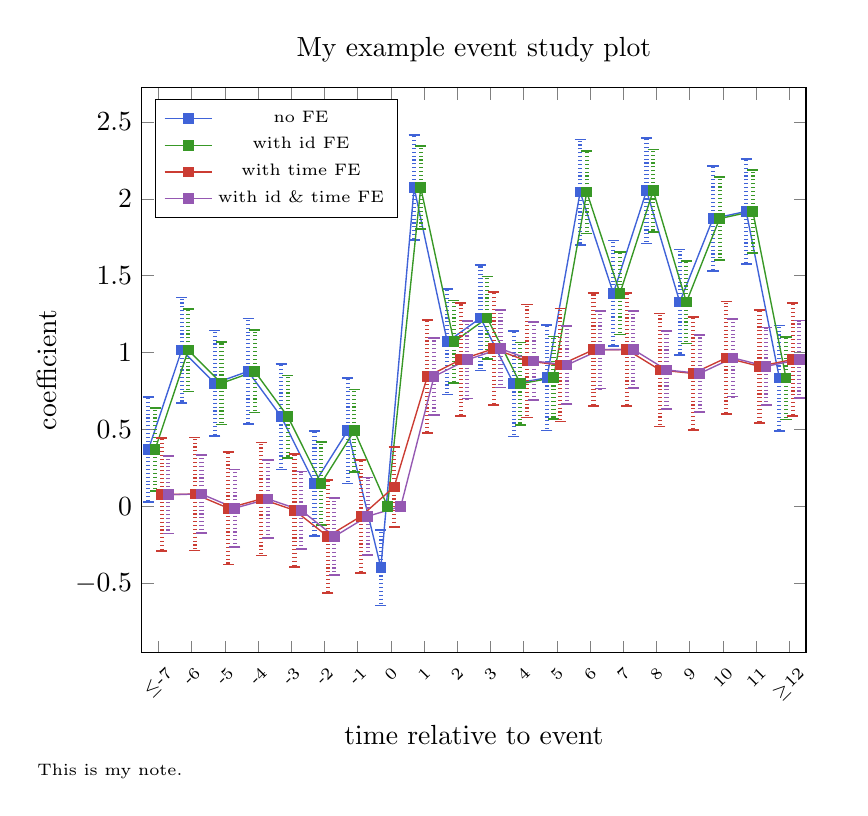
\begin{tikzpicture}
\begin{axis}[title={My example event study plot}, title style={}, xlabel={time relative to event}, xlabel style={}, ylabel={coefficient}, ylabel style={}, xticklabel style={font={\fontsize{6}{6}\selectfont}, rotate={45}}, yticklabel style={}, width={240pt}, height={204pt}, legend style={font={\fontsize{6}{6}\selectfont}, at={(0.02, 0.98)}, anchor={north west}}, symbolic x coords={$\leq$-7,-6,-5,-4,-3,-2,-1,0,1,2,3,4,5,6,7,8,9,10,11,$\geq$12}, xtick={$\leq$-7,-6,-5,-4,-3,-2,-1,0,1,2,3,4,5,6,7,8,9,10,11,$\geq$12}, xmin={{[normalized]-0.5}}, xmax={{[normalized]19.5}}, scale only axis]
    \addplot[mark={square*}, mark options={mark size={1.75pt}, line width={0pt}, fill={rgb,255: red, 64; green, 99; blue, 216}, fill opacity={1}, draw={rgb,255: red, 64; green, 99; blue, 216}, draw opacity={1}}, error bars/error mark={|}, error bars/error mark options={mark size={2.0pt}, solid, line width={0.6pt}, fill={rgb,255: red, 64; green, 99; blue, 216}, fill opacity={1}, draw={rgb,255: red, 64; green, 99; blue, 216}, draw opacity={1}}, error bars/error bar style={draw={rgb,255: red, 64; green, 99; blue, 216}, draw opacity={1}, densely dotted, line width={1.5pt}}, draw={rgb,255: red, 64; green, 99; blue, 216}, draw opacity={1}, line width={0.5pt}, error bars/y dir={both}, error bars/y explicit, x filter/.code={{\pgfmathadd{\pgfmathresult}{-0.30000000000000004}}}]
        coordinates {
            ($\leq$-7,0.36968848040219676) +- (0,0.34266703123022935)
            (-6,1.016164254335906) +- (0,0.34266703123022935)
            (-5,0.800435137464947) +- (0,0.3426670312302293)
            (-4,0.8778993522840294) +- (0,0.34266703123022935)
            (-3,0.5827695112478368) +- (0,0.34266703123022946)
            (-2,0.14944225350719761) +- (0,0.34266703123022935)
            (-1,0.49160731109998046) +- (0,0.34266703123022935)
            (0,-0.39846952781006556) +- (0,0.2453653895616492)
            (1,2.0726463666986454) +- (0,0.34266703123022935)
            (2,1.0699196982728019) +- (0,0.34266703123022935)
            (3,1.2250710642967737) +- (0,0.34266703123022935)
            (4,0.7976719857020569) +- (0,0.34266703123022935)
            (5,0.8364708751690804) +- (0,0.34266703123022935)
            (6,2.04374488079733) +- (0,0.34266703123022935)
            (7,1.385907470897243) +- (0,0.34266703123022935)
            (8,2.0529242306768922) +- (0,0.34266703123022935)
            (9,1.3283311252365138) +- (0,0.34266703123022935)
            (10,1.8713616815794052) +- (0,0.34266703123022935)
            (11,1.9179877639249006) +- (0,0.34266703123022935)
            ($\geq$12,0.8338398361406821) +- (0,0.34266703123022935)
        }
        ;
    \addlegendentry {no FE}
    \addplot[mark={square*}, mark options={mark size={1.75pt}, line width={0pt}, fill={rgb,255: red, 56; green, 152; blue, 38}, fill opacity={1}, draw={rgb,255: red, 56; green, 152; blue, 38}, draw opacity={1}}, error bars/error mark={|}, error bars/error mark options={mark size={2.0pt}, solid, line width={0.6pt}, fill={rgb,255: red, 56; green, 152; blue, 38}, fill opacity={1}, draw={rgb,255: red, 56; green, 152; blue, 38}, draw opacity={1}}, error bars/error bar style={draw={rgb,255: red, 56; green, 152; blue, 38}, draw opacity={1}, densely dotted, line width={1.5pt}}, draw={rgb,255: red, 56; green, 152; blue, 38}, draw opacity={1}, line width={0.5pt}, error bars/y dir={both}, error bars/y explicit, x filter/.code={{\pgfmathadd{\pgfmathresult}{-0.10000000000000003}}}]
        coordinates {
            ($\leq$-7,0.3696884804022053) +- (0,0.2685897091663007)
            (-6,1.0161642543359157) +- (0,0.2685897091663007)
            (-5,0.8004351374649559) +- (0,0.2685897091663007)
            (-4,0.8778993522840397) +- (0,0.26858970916630076)
            (-3,0.5827695112478463) +- (0,0.26858970916630076)
            (-2,0.14944225350720666) +- (0,0.26858970916630076)
            (-1,0.4916073110999887) +- (0,0.26858970916630076)
            (0,0.0) +- (0,0.0)
            (1,2.0726463666986557) +- (0,0.2685897091663007)
            (2,1.0699196982728107) +- (0,0.2685897091663007)
            (3,1.2250710642967848) +- (0,0.2685897091663007)
            (4,0.7976719857020667) +- (0,0.26858970916630076)
            (5,0.836470875169089) +- (0,0.2685897091663007)
            (6,2.043744880797339) +- (0,0.26858970916630065)
            (7,1.385907470897252) +- (0,0.2685897091663007)
            (8,2.0529242306769) +- (0,0.2685897091663006)
            (9,1.3283311252365224) +- (0,0.26858970916630076)
            (10,1.8713616815794152) +- (0,0.2685897091663008)
            (11,1.9179877639249088) +- (0,0.26858970916630076)
            ($\geq$12,0.8338398361406912) +- (0,0.26858970916630076)
        }
        ;
    \addlegendentry {with id FE}
    \addplot[mark={square*}, mark options={mark size={1.75pt}, line width={0pt}, fill={rgb,255: red, 203; green, 60; blue, 51}, fill opacity={1}, draw={rgb,255: red, 203; green, 60; blue, 51}, draw opacity={1}}, error bars/error mark={|}, error bars/error mark options={mark size={2.0pt}, solid, line width={0.6pt}, fill={rgb,255: red, 203; green, 60; blue, 51}, fill opacity={1}, draw={rgb,255: red, 203; green, 60; blue, 51}, draw opacity={1}}, error bars/error bar style={draw={rgb,255: red, 203; green, 60; blue, 51}, draw opacity={1}, densely dotted, line width={1.5pt}}, draw={rgb,255: red, 203; green, 60; blue, 51}, draw opacity={1}, line width={0.5pt}, error bars/y dir={both}, error bars/y explicit, x filter/.code={{\pgfmathadd{\pgfmathresult}{0.09999999999999998}}}]
        coordinates {
            ($\leq$-7,0.07645489065628518) +- (0,0.3671540529718498)
            (-6,0.07996822101712148) +- (0,0.3671540529718497)
            (-5,-0.011650219338167655) +- (0,0.3671540529718498)
            (-4,0.04827405540176742) +- (0,0.36715405297184966)
            (-3,-0.025795428786320893) +- (0,0.36715405297184983)
            (-2,-0.19579864129185184) +- (0,0.3671540529718498)
            (-1,-0.06466735007183572) +- (0,0.3671540529718498)
            (0,0.12688902752253867) +- (0,0.2596171205965209)
            (1,0.8447808240898926) +- (0,0.36715405297184983)
            (2,0.9532945471851118) +- (0,0.3671540529718497)
            (3,1.0256382459735547) +- (0,0.3671540529718497)
            (4,0.9454918497954906) +- (0,0.3671540529718498)
            (5,0.9192463471134921) +- (0,0.36715405297184983)
            (6,1.0183105850288396) +- (0,0.3671540529718498)
            (7,1.0200496824371605) +- (0,0.36715405297184966)
            (8,0.8870106225498702) +- (0,0.3671540529718497)
            (9,0.8643245121103159) +- (0,0.3671540529718498)
            (10,0.9657067575074176) +- (0,0.36715405297184966)
            (11,0.910557345992743) +- (0,0.3671540529718497)
            ($\geq$12,0.955515325711472) +- (0,0.3671540529718497)
        }
        ;
    \addlegendentry {with time FE}
    \addplot[mark={square*}, mark options={mark size={1.75pt}, line width={0pt}, fill={rgb,255: red, 149; green, 88; blue, 178}, fill opacity={1}, draw={rgb,255: red, 149; green, 88; blue, 178}, draw opacity={1}}, error bars/error mark={|}, error bars/error mark options={mark size={2.0pt}, solid, line width={0.6pt}, fill={rgb,255: red, 149; green, 88; blue, 178}, fill opacity={1}, draw={rgb,255: red, 149; green, 88; blue, 178}, draw opacity={1}}, error bars/error bar style={draw={rgb,255: red, 149; green, 88; blue, 178}, draw opacity={1}, densely dotted, line width={1.5pt}}, draw={rgb,255: red, 149; green, 88; blue, 178}, draw opacity={1}, line width={0.5pt}, error bars/y dir={both}, error bars/y explicit, x filter/.code={{\pgfmathadd{\pgfmathresult}{0.3}}}]
        coordinates {
            ($\leq$-7,0.07645489065628643) +- (0,0.2521561516835071)
            (-6,0.07996822101712256) +- (0,0.2521561516835071)
            (-5,-0.01165021933816684) +- (0,0.2521561516835071)
            (-4,0.04827405540176775) +- (0,0.2521561516835071)
            (-3,-0.02579542878631976) +- (0,0.2521561516835071)
            (-2,-0.19579864129185118) +- (0,0.2521561516835071)
            (-1,-0.0646673500718346) +- (0,0.2521561516835071)
            (0,0.0) +- (0,0.0)
            (1,0.8447808240898917) +- (0,0.2521561516835071)
            (2,0.9532945471851113) +- (0,0.2521561516835071)
            (3,1.0256382459735534) +- (0,0.25215615168350713)
            (4,0.9454918497954905) +- (0,0.2521561516835071)
            (5,0.9192463471134917) +- (0,0.2521561516835071)
            (6,1.018310585028839) +- (0,0.2521561516835071)
            (7,1.0200496824371603) +- (0,0.2521561516835071)
            (8,0.8870106225498696) +- (0,0.2521561516835071)
            (9,0.8643245121103146) +- (0,0.252156151683507)
            (10,0.9657067575074167) +- (0,0.252156151683507)
            (11,0.910557345992743) +- (0,0.2521561516835071)
            ($\geq$12,0.9555153257114705) +- (0,0.252156151683507)
        }
        ;
    \addlegendentry {with id \& time FE}
\end{axis}
\newdimen\notewidth
                    \pgfextractx{\notewidth}{\pgfpointdiff{\pgfpointanchor{current bounding box}{west}}
                    {\pgfpointanchor{current bounding box}{east}}}\draw node[text width={\the\notewidth}, anchor={north west}, at={(current axis.outer south west)}, align={left}, font={\fontsize{6}{6}\selectfont}] {This is my note.};
\end{tikzpicture}
\end{document}
